%!TEX root = report.tex

\chapter{The C3AE Model}
\label{chp:theorystuff}

\section{Model details}

The C3AE plain model takes as input a source image and tries to output a plausible estimation for the 
age of the portrayed person.

Since the objective is to obtain a lightweight model the total number of parameters needs to be as low 
as possible, as long as it doesn't affect the overall performance. 
For this reason the input image size is limited (64×64×3) and the other channels sizes are also small.\\
Standard convolutional layers are adequate for the trade-off between accuracy and compactness (as 
opposed to the separable convolution block used in the bigger models like MobileNets and ShuffleNets), 
followed by batch normalization, Relu and average pooling (BRA).\\
The model is composed of five of these standard convolutions and two fully connected layers as shown 
in \autoref{tab:architecture}.

\begin{center}
    \begin{tabular}{||c | c c c c||} 
    \hline
    Layer & Kernel & Stride & Output size & Parameters \\ 
    \hline\hline
    Image & - & 1 & 64×64×3 & - \\
    \hline
    Conv. 1 & 3×3×32 & 1 & 62×62×32 & 896 \\
    \hline
    BRA & - & 1 & 31×31×32 & 128 \\
    \hline
    Conv. 2 & 3×3×32 & 1 & 29×29×32 & 9248 \\
    \hline
    BRA & - & 1 & 14×14×32 & 128 \\ 
    \hline
    Conv. 3 & 3×3×32 & 1 & 12×12×32 & 9248 \\ 
    \hline
    BRA & - & 1 & 6×6×32 & 128 \\ 
    \hline
    Conv. 4 & 3×3×32 & 1 & 4×4×32 & 9248 \\ 
    \hline
    BN + ReLu & - & 1 & 4×4×32 & 128 \\ 
    \hline
    Conv5 & 1×1×32 & 1 & 4×4×32 & 1056 \\ 
    \hline
    Feat. & 1×1×32 & 1 & 12 & 6156 \\ 
    \hline
    Predict. & 1×1×1 & 1 & 1 & 13 \\ 
    \hline
    \end{tabular}
    \captionof{table}{Architecture of the model}
    \label{tab:architecture}
\end{center}

To estimate people's age C3AE considers two objectives simultaneously: the first one minimizes the 
Kullback-Leibler loss between distributions, and the second one optimizes the squared loss between 
discrete ages.

In the following sections are mentioned this and other techniques used in C3AE.

\begin{figure}[!ht]
    \centering
    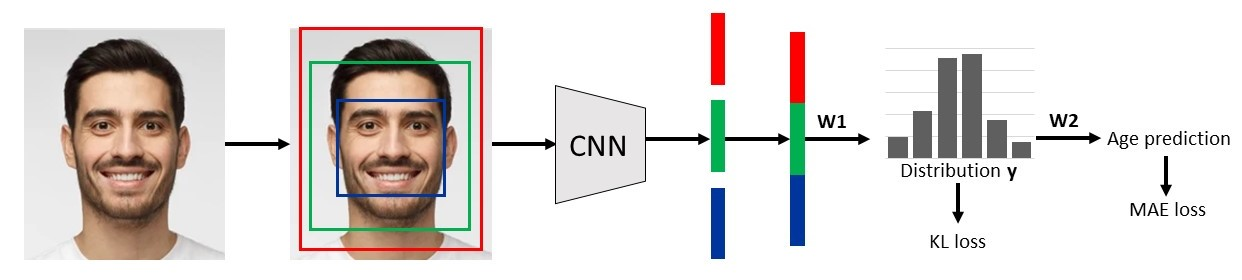
\includegraphics[width=400pt]{images/model.jpg}
    \caption{Overview of the model age estimation process}
    \label{fig:overview}
\end{figure}

\subsection*{Context-based Regression}
The resolution and the size of small-scale image is limited, so the idea is to exploit facial information 
at different granularity levels. 
After the face recognition task we identify three different crops of different sizes of the subject's face, 
like in Figure 3.1. Each cropped image has a special view on the face. 
The smaller image contains rich local information; in return the bigger one may contain global and scene 
information.
The three crops are then fed into the shared CNN network, and finally the bottlenecks of the
three-scale facial images are aggregated by concatenation.

\subsection*{Two-point Age Representation}
With C3AE we don't predict directly the age as a number. Instead, this model uses a two-point age 
representation through a distribution over two discrete adjacent bins.\\
For example let's consider the corresponding representation of an age of 22 with 10 bins. In this 
case the set of bins is [10, 20, 30, 40, 50, 60, 70, 80, 90, 100] and the corresponding vector 
representation of the age is [0, 0.8, 0.2, 0, 0, 0, 0, 0, 0, 0].

\subsection*{Cascade Training}
From the above section, the age value can be represented as a distribution vector. The mapping from this 
vector to age value is decomposed into two steps, where we define two different losses for the two cascade 
tasks.\\
The first one ($L_{kl}$) measures the discrepancy between ground-truth label and predicted age distribution.
We adopt KL-Divergence as the measurement.\\
The second loss ($L_{reg}$) controls the prediction of the final age and is implemented as an L1 distance
or mean absolute error (MAE loss).\\
In the training process the two loss functions are considered in the cascade style as shown in Figure 3.1 
but they are still trained jointly, and the total loss is given as
$L_{total} = \alpha L_{kl} + L_{reg}$, where $\alpha$ is the hyperparameter to balance the two losses.

\section{Implementation}
Our implementation of the C3AE model can be found on
GitHub.\footnote{\url{https://github.com/torchipeppo/C3AE-tf2}}
The code for this part of the project is based on the Tensorflow library for Python and was written in 
Visual Studio Code text editor, collaborating remotely using the Live Share extension feature, which let 
us write the code together.
\subsection*{The model}
The code of the model implementation can be found in the directory \texttt{master/model.py}. We followed 
as strictly as possible the structure indicated in the reference paper, both in the number, composition 
and ordering of the layers and also in the choice of parameters such as kernel dimensions, bottleneck
dimension and squeeze factors.
The Keras package integrated in Tensorflow provided all the basic functions needed to implement the
building blocks of the C3AE plain model, shared by all three of the image cuts.


In the last part of the file we organized the code so that we could be able to replicate the ablation
studies conducted in the original C3AE paper. Ablation studies are procedure where certain parts of the 
network are removed, in order to gain a better understanding of the network’s behaviour. In our case, 
the two ablations affect the presence or the absence of the cascade module and the context module.
The \texttt{model.py} file therefore gives us the possibility to analize not only the full context 
model, but also compare it with three slightly simpler ones: the model without cascade, without context 
and without both.

The presence of these alternative versions required some changes in the code:

\begin{itemize}
    \item \textit{Context ablation}: produces only one simple input, instead of three concatenated ones, 
    before computing the losses in the training phase. This means we will train using only one cut of the 
    photos, the outer one.
    \item \textit{Cascade ablation}: in this case we lose the concept of two-point age representation.
    We replace the last dense layer W1 with a hidden layer with no particular meaning and then only
    considered one output, the age prediction, and ignore the second output, the age distribution.
    It follows thatin the training phase we will only evaluate the MAE loss in this case, since the KL 
    divergence loss will no longer be present. 
    \item \textit{Full ablation}: both of the above modifications apply.
\end{itemize}

The results of these ablation studies are discussed later in \fullref{sec:ablation_study}.

\subsection*{The training}
The code relevant to the training phase can be found in \texttt{master/training.py}. Again, the choice of
the parameters such as learning rate, batch sizes and optimizers follows the values indicated in the source 
paper when possible, with a couple of exceptions.

The dataset split ratio into training and validation was not specified for the datasets we used, so we 
chose a value of 88\% - 12\%.

In the original paper for a comparison with the state-of-the-art methods, each model has been trained for 
600 epochs. In our implementation this number had to be cut down to 100, the reason being time constraints 
and hardware availability. All training was conducted locally on a machine with a Nvidia GTX 1660 SUPER GPU, 
and even with 100 epochs each training phase lasted for 10 hours on average. A discussion on how this 
cutback may not have affected the final results is present in the next chapter.

In this section of the code we also implemented the possibility to take an already trained model and continue
its training on another dataset, instead of starting over from zero. An experiment taking advantage of this 
feature is described in \fullref{subsec:wikiutk}.



